\subsection{Intro und Outro}
\mysubsubsection{Fabian Gärtner}{Technik}

Die Bilder zum Intro und Outro befinden sich im Anhang (siehe ab \ref{Intro}).

Das Spiel soll von Anfang an den Spieler zur Hauptrolle machen, weshalb das Intro und Outro so gestaltet wurde, dass es dem Spieler deutlich vermittelt, dass er persönlich vom verrücken Wissenschaftler zu Hilfe gerufen wurde. Wenn der Spieler das Spiel startet und die Brille aufsetzt, sieht er daher zunächst - nach einem Ladebildschirm - über die Kamera des Smartphones die Realwelt vor sich. Ein Text auf dem Bildschirm erklärt anschließend, dass der Spieler nun seinen magischen Würfel wie gezeigt (mit dem Stern zur Kamera) in das Bild halten soll. Tut er dies für fünf Sekunden, beginnt eine Sequenz, die den Spieler aus der Realwelt in die Spielwelt teleportiert. Auch hier wird das Spiel der Themenvorgabe gerecht, da der Spieler eine Reise von der Realität in die virtuelle Welt, also zwischen verschiedenen Dimensionen, miterlebt. Vermittelt wird dem Spieler diese Reise visuell durch das Einfrieren, Drehen, Verschwimmen und Überlichten des Kamerabildes und das anschließende Einblenden einer drehenden Spirale. Gleichzeitig wird diese Sequenz als eine Einleitung in das Spiel genutzt, indem dem Spieler die Vorgeschichte visuell über sechs hereinfliegende Comics und auditiv durch einen Erzähler vermittelt wird. Nach diesem Intro landet der Spieler innerhalb des dunklen Würfels und kann mit der Erkundung der Welt beginnen.

Das Outro beginnt, sobald der Spieler alle Rätsel gelöst hat. Da nun der Remote Cube wieder zusammengesetzt und funktionsfähig ist, beginnt sich die Welt um den Spieler herum aufzuklappen und eine Insel zu bilden. Zum ersten Mal sieht der Spieler dadurch den Bereich außerhalb des Würfels, der vor allem durch seine Low-Poly-Skybox auffällt, die sowohl den Himmel als auch das Wasser um die aufgeklappte Würfel-Welt herum darstellt und ebenfalls eine würfelartige Form hat. Des Weiteren erkennt der Spieler nun, da er von oben auf den aufgeklappten Würfel schaut, dass diese Welt tatsächlich auch als Insel die Form eines Würfels hat und kann daher nachvollziehen, warum der verrückte Wissenschaflter derartige Vermutungen hatte. Nach zehn Sekunden beginnt dann das Bild zu überlichten und die Rückreise für den Spieler steht an. Während der drehenden Spirale dankt der verrücke Wissenschaftler dem Spieler erneut auditiv während wiederum Comics sowohl die Story komplettieren, als auch den Abspann für das Spiel bilden. Anschließend überblendet das Spiel noch einmal und der Spieler sieht wieder das reale Kamerabild - er ist also zurück in der Realität.


\mysubsubsection{Sandra Beuck}{Art}

\begin{figure}[!htbp]%[htbp]
	\centering
		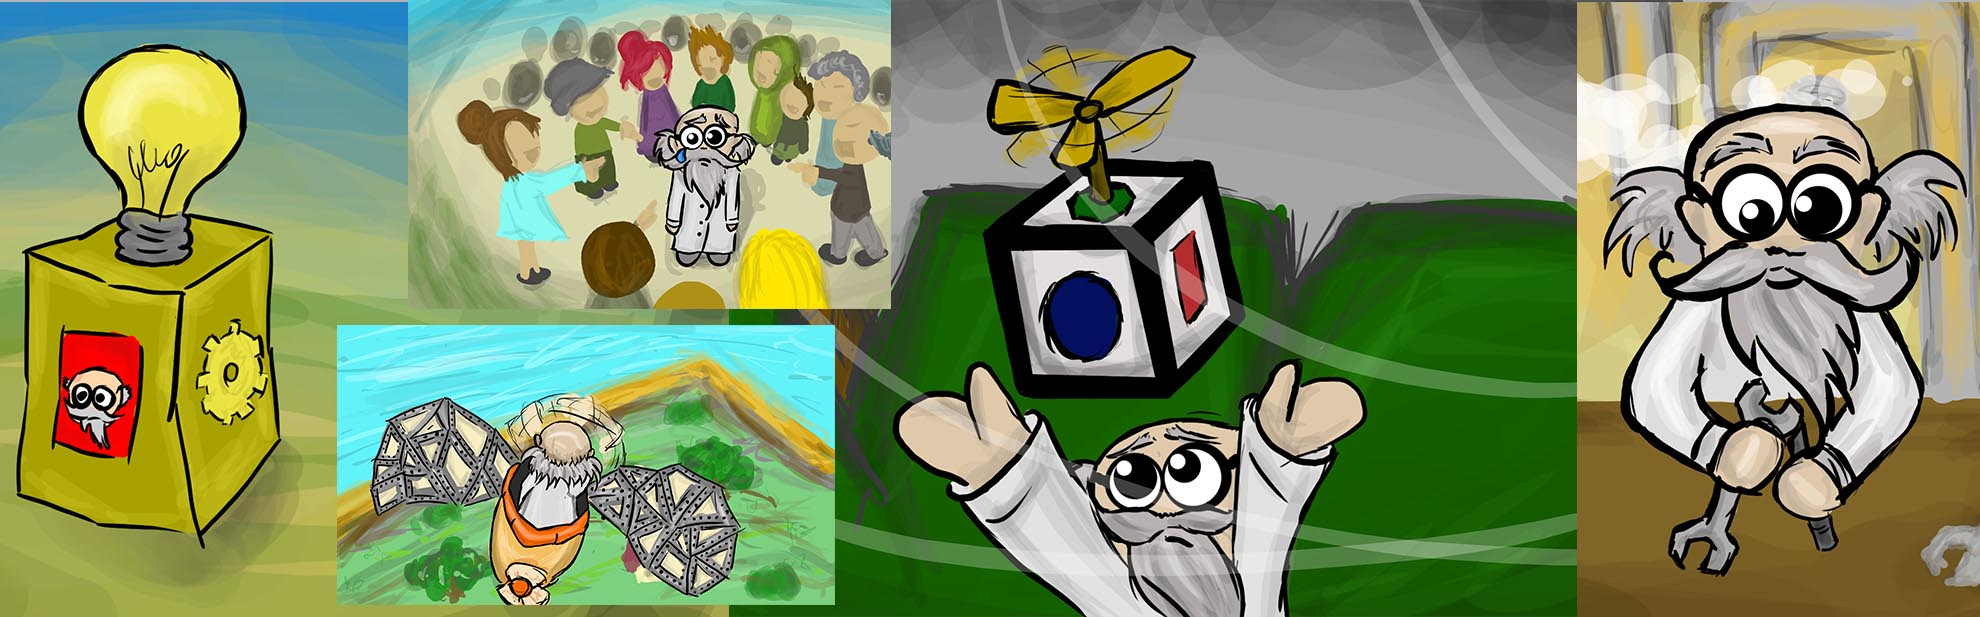
\includegraphics[width=0.9\textwidth]{images/illustrationen}
	\caption{Illustrationen}
	\label{fig:Illustrationen}
\end{figure}

Um den Spieler in das Spiel einzuführen dient das Intro. Es besteht aus sechs Einzelbildern, die in Photoshop mit Hilfe eines Grafiktabletts gezeichnet wurden. Die Erzählung des verrückten Wissenschaftlers wird durch den Dialog und in Bildern ausgedrückt. Dabei steht er durch die betonten Konturen, im Gegensatz zum Hintergrund besonders im Vordergrund. Dies leitet den Spieler in seiner Blickführung. Der Stil der Zeichnungen ist an das Low-Poly Thema angepasst, interpretiert es aber neu in einem Comicstil.

Das Outro führt den Spieler aus dem Spiel. Es zeigt den Würfel, der sich zusammensetzt. Es besteht aus drei Einzelbildern, von denen zwei den Würfel zeigen und eines die Credits. Der verrückte Wissenschaftler wird bewusst nicht mehr gezeigt, denn das Ziel des Spieles ist erreicht und der Würfel steht im Fokus der Aufmerksamkeit. Deshalb ist der Hintergrund bewusst simpel gestaltet.